% !TeX encoding = UTF-8
\documentclass[aspectratio=169]{beamer}
\useoutertheme[progressbar=frametitle]{metropolis}
\useinnertheme{metropolis}
\definecolor{nabgray}{rgb}{0.6,0.59,0.61}
\usecolortheme[named=nabgray]{structure}
\usepackage{fontawesome5}
\usepackage{tikz}
\usepackage[utf8]{inputenc}
\usepackage[spanish]{babel}
\usepackage{fontspec}
\setmonofont{JetBrains Mono}
\setmainfont{Helvetica Neue}
\setsansfont{Helvetica Neue}

\usepackage{smartdiagram}
\usepackage{qtree}
\usepackage{verbatim}
\usepackage{svg}
\usepackage{graphicx}
\usepackage{color}

\definecolor{lightgray}{rgb}{0.95, 0.95, 0.95}
\definecolor{darkgray}{rgb}{0.4, 0.4, 0.4}
%\definecolor{purple}{rgb}{0.65, 0.12, 0.82}
\definecolor{editorGray}{rgb}{0.95, 0.95, 0.95}
\definecolor{editorOcher}{rgb}{1, 0.5, 0} % #FF7F00 -> rgb(239, 169, 0)
\definecolor{editorGreen}{rgb}{0, 0.5, 0} % #007C00 -> rgb(0, 124, 0)
\definecolor{orange}{rgb}{1,0.45,0.13}
\definecolor{olive}{rgb}{0.17,0.59,0.20}
\definecolor{brown}{rgb}{0.69,0.31,0.31}
\definecolor{purple}{rgb}{0.38,0.18,0.81}
\definecolor{lightblue}{rgb}{0.1,0.57,0.7}
\definecolor{lightred}{rgb}{1,0.4,0.5}
\usepackage{upquote}
\usepackage{listings}
\lstset{language=java,
	basicstyle=\footnotesize\ttfamily,
	keywordstyle=\footnotesize\color{blue}\ttfamily,
	escapeinside={<@}{@>}
}

\usebackgroundtemplate%
{%
	
\includegraphics[width=\paperwidth]{Images/Contenido}%
}

\title{OpenTelemetry: La lingua franca de la observabilidad}
\subtitle{No puedes mejorar lo que no puedes medir}
\author{Nabenik}
\date{\today}

\begin{document}
	
	{
		\usebackgroundtemplate{
\includegraphics[width=\paperwidth]{Images/portada}}
		\begin{frame}
			\maketitle
		\end{frame}
	}
	
	\begin{frame}{La realidad Cloud Native}
		
		\begin{itemize}
			\item Cargas de trabajo potenciadas por Internet
			\item Cargas de trabajo elásticas
			\item Cargas de trabajo en capas y abstracciones (Kubernetes, Docker)
		\end{itemize}		
		
	\end{frame}
	
	\begin{frame}{Observabilidad y monitoreo}
		
		\begin{columns}
			
			\begin{column}{0.5\textwidth}
				Sistema informático {\Huge \faServer}
				\begin{itemize}
					\item Aplicaciones
					\item Servicios de terceros
					\item Procesos
					\item Hosts
				\end{itemize}
			\end{column}
			
			\begin{column}{0.5\textwidth}
				{\Huge	 \faBinoculars}
			\end{column}
		\end{columns}
		
	\end{frame}
	
	\begin{frame}{Observabilidad y monitoreo}
		
		\begin{columns}
			
			\begin{column}{0.5\textwidth}
				Sistema informático {\Huge \faServer}
				\begin{itemize}
					\item Aplicaciones
					\item Servicios de terceros
					\item Procesos
					\item Hosts
				\end{itemize}
			\end{column}
			
			\begin{column}{0.5\textwidth}
				Fuentes de información {\Huge	 \faBinoculars}
				\begin{itemize}
					\item Eventos
					\item Traces
					\item Logs
					\item Métricas
				\end{itemize}
			\end{column}
		\end{columns}
		
	\end{frame}
	
	\begin{frame}{La observabilidad clásica}
		
		Application server
		\begin{itemize}
			\item Logs - systemd, /opt/tomcat/logs
			\item Métricas - Rendimiento de JVM (JMX)
			\item Tracing - Glimpse, Zipkin
		\end{itemize}
		
	\end{frame}
	
	{
		\usebackgroundtemplate{
\includegraphics[width=\paperwidth]{Images/separador}}
		\setbeamercolor{normal text}{fg=white}
		\setbeamercolor{frametitle}{fg=red}
		\usebeamercolor[fg]{normal text}
		\section{Fuentes de datos}
	}
	
	\begin{frame}{Métricas}
		
		\begin{block}{Definición}
			Valores numéricos sobre el rendimiento de las aplicaciones -e.g. Rendimiento de red, tamaño del heap-
		\end{block}	
		Formatos
		\begin{itemize}
			\item Gauge (instantáneas)
			\item Delta (diferencia entre dos puntos)
			\item Acumulativas (cambios en el tiempo)
		\end{itemize}
		
		Modo clásico
		\begin{itemize}
			\item OS
			\item JMX
			\item Http Endpoint (/actuator/metrics)
		\end{itemize}	
	\end{frame}
	
	\begin{frame}
		\begin{figure}
			\centering
			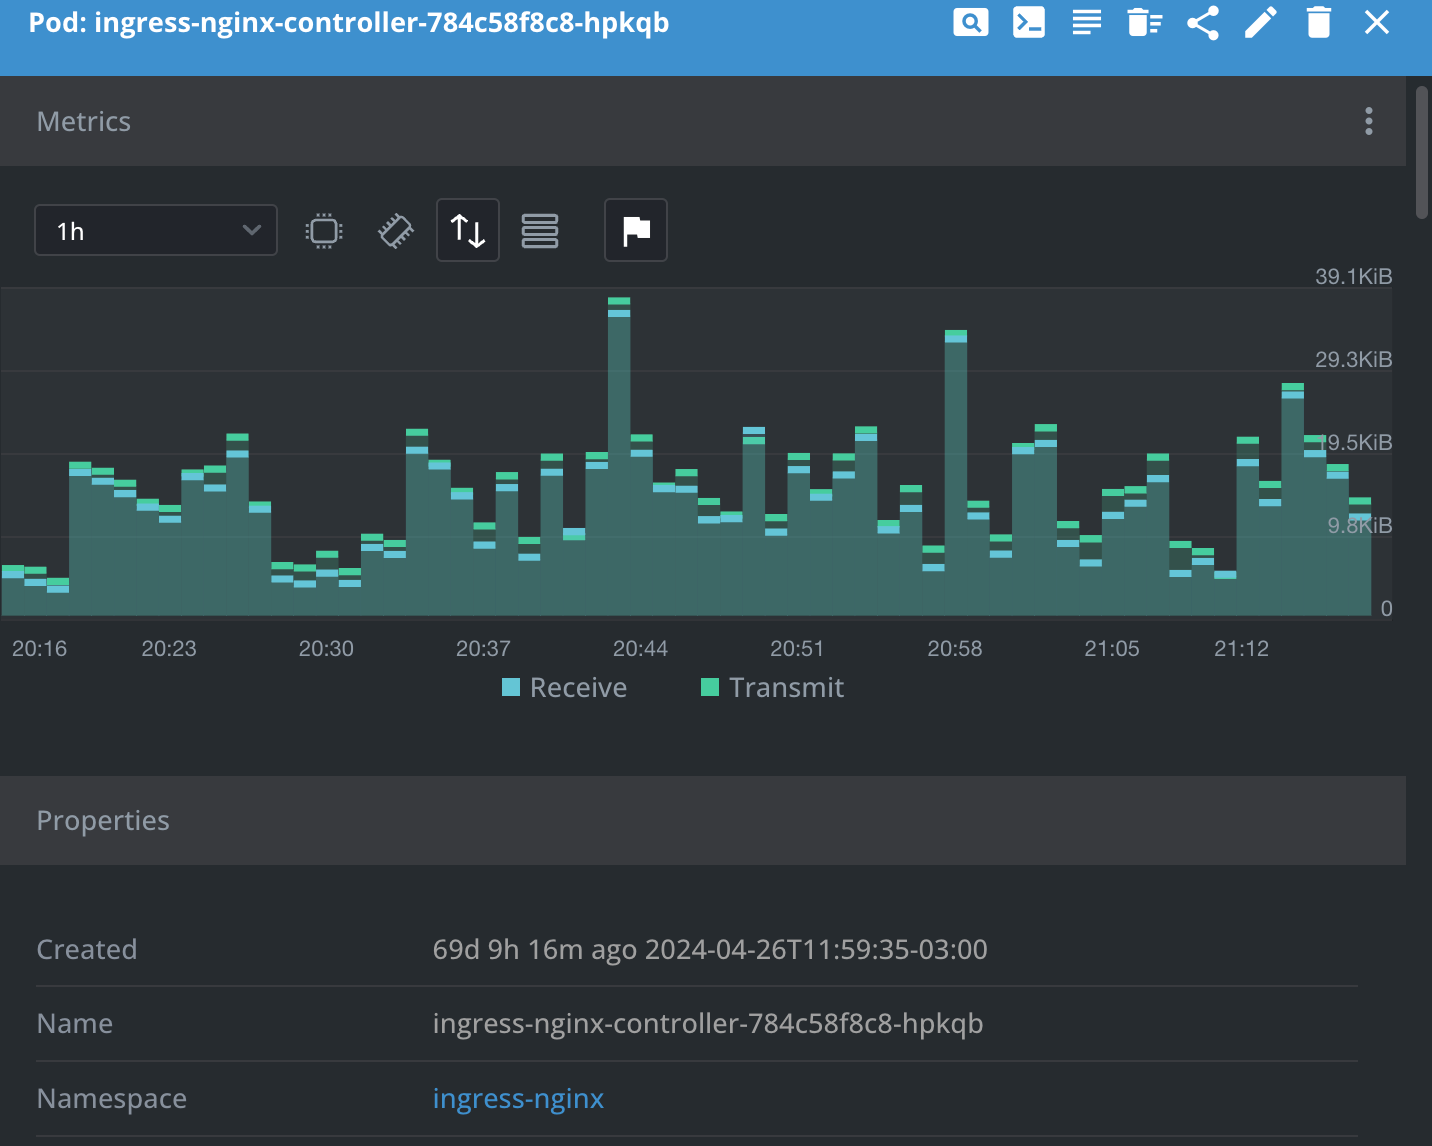
\includegraphics[width=0.7\linewidth]{Images/metrics-sample}
			\label{fig:metrics-sample}
		\end{figure}
	\end{frame}
	
	\begin{frame}{Logs}
		
		\begin{block}{Definición}
			Registro histórico de procesos, eventos y mensajes con datos adicionales como timestamps y contexto
		\end{block}	
		Modo clásico
		\begin{itemize}
			\item Archivos en el sistema
			\item SystemD
			\item FluentD
		\end{itemize}	
	\end{frame}
	
	\begin{frame}
		\begin{figure}
			\centering
			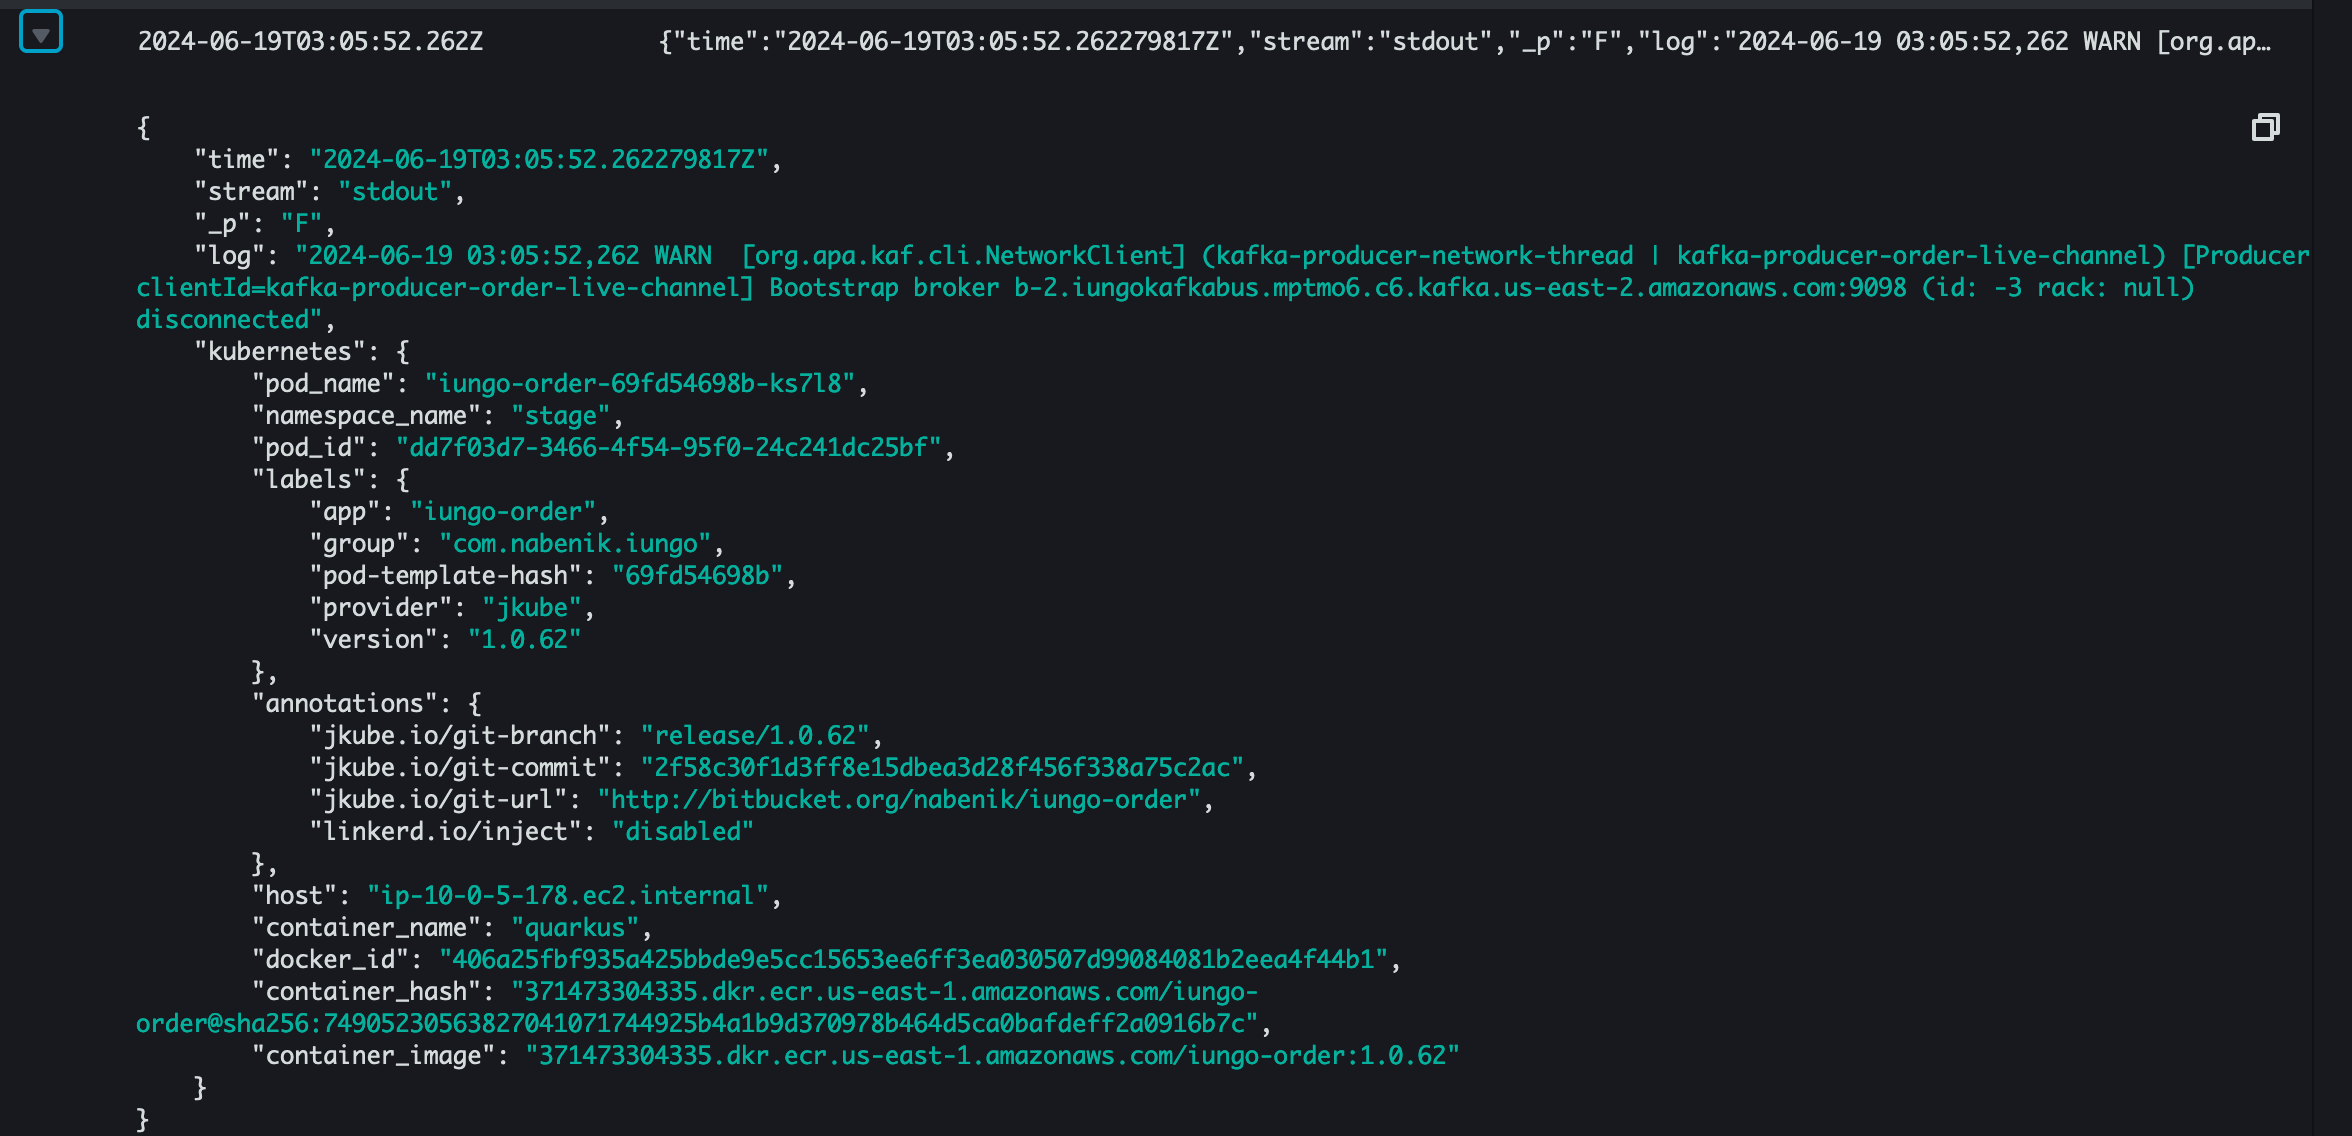
\includegraphics[width=0.8\linewidth]{Images/logs-sample}
			\label{fig:logs-sample}
		\end{figure}
	\end{frame}
	
	\begin{frame}{Trace}
		
		\begin{block}{Definición}
			Ruta completa de una operación dentro de una serie de sistemas interrelacionados. Cada participante crea spans que en conjunto se convierten en traces
		\end{block}	
		Modo clásico
		\begin{itemize}
			\item Protocolos de push propietarios -e.g. Jaeger, Zipkin-
		\end{itemize}	
	\end{frame}
	
	\begin{frame}
		\begin{figure}
			\centering
			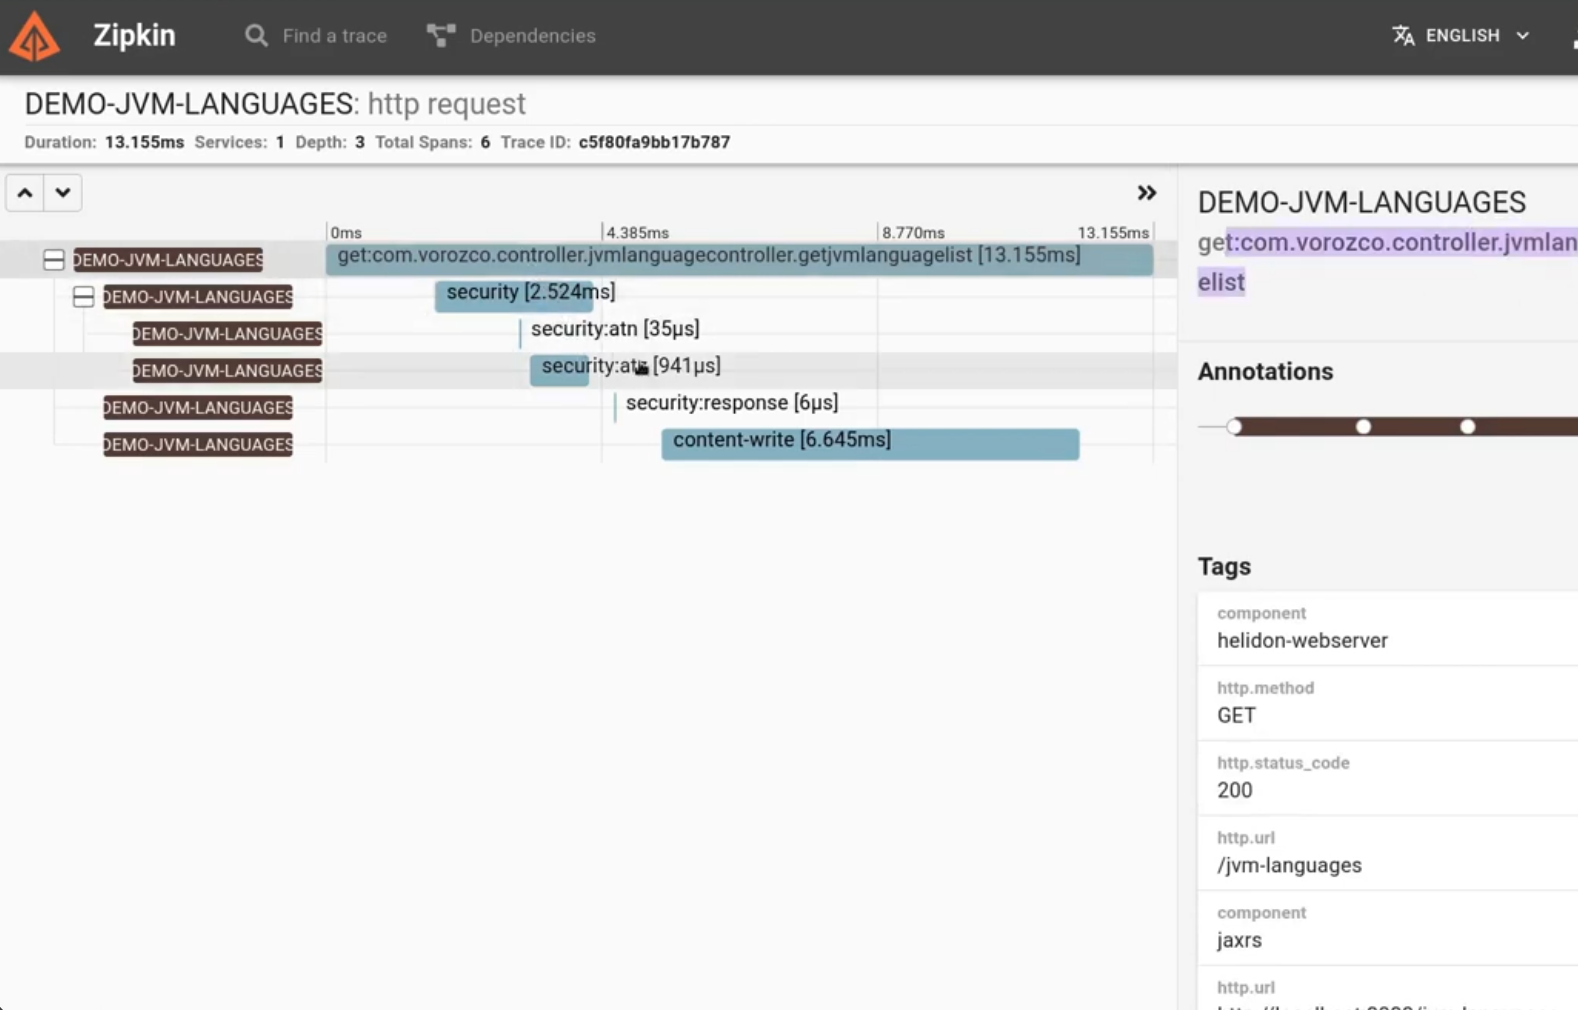
\includegraphics[width=0.7\linewidth]{Images/trace-sample}
			\label{fig:trace-sample}
		\end{figure}
	\end{frame}
	
	{
		\usebackgroundtemplate{
\includegraphics[width=\paperwidth]{Images/separador}}
		\setbeamercolor{normal text}{fg=white}
		\setbeamercolor{frametitle}{fg=red}
		\usebeamercolor[fg]{normal text}
		\section{OpenTelemetry}
	}
	
	\begin{frame}
		\begin{figure}
			\centering
			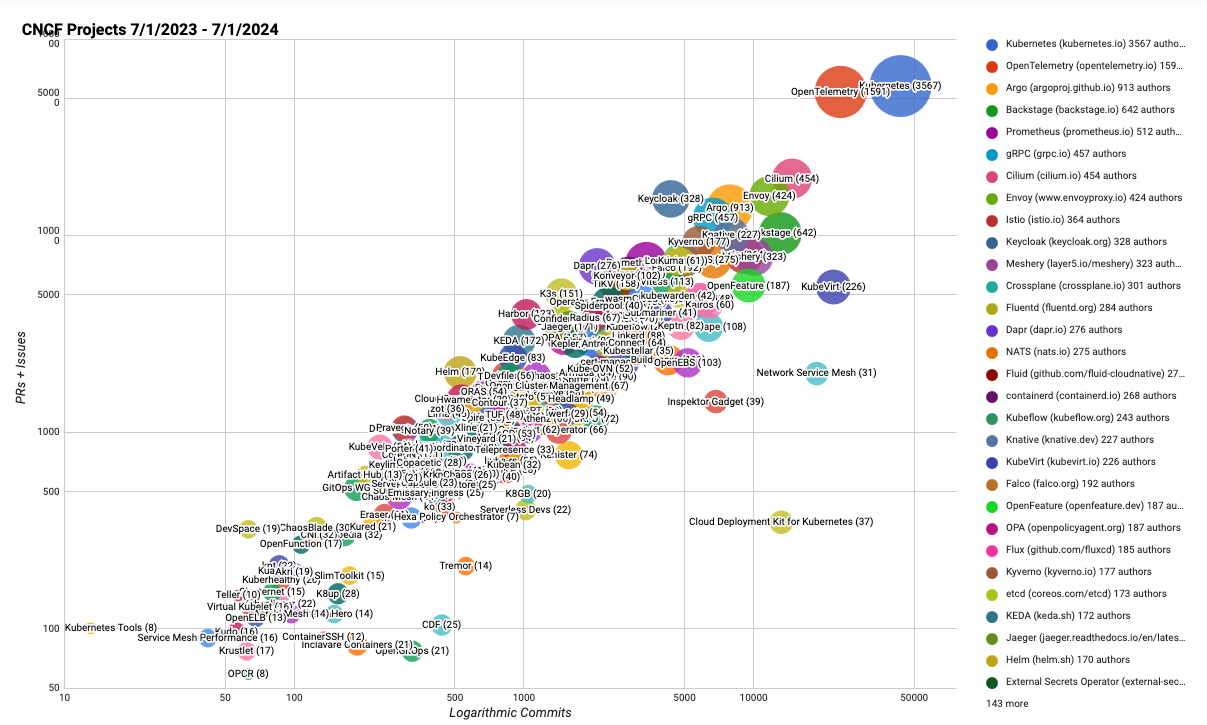
\includegraphics[width=0.9\linewidth]{Images/cncfprojects}
			\label{fig:cncfprojects}
		\end{figure}
	\end{frame}
	
	\begin{frame}{OpenTelemetry}
		\begin{figure}
			\centering
			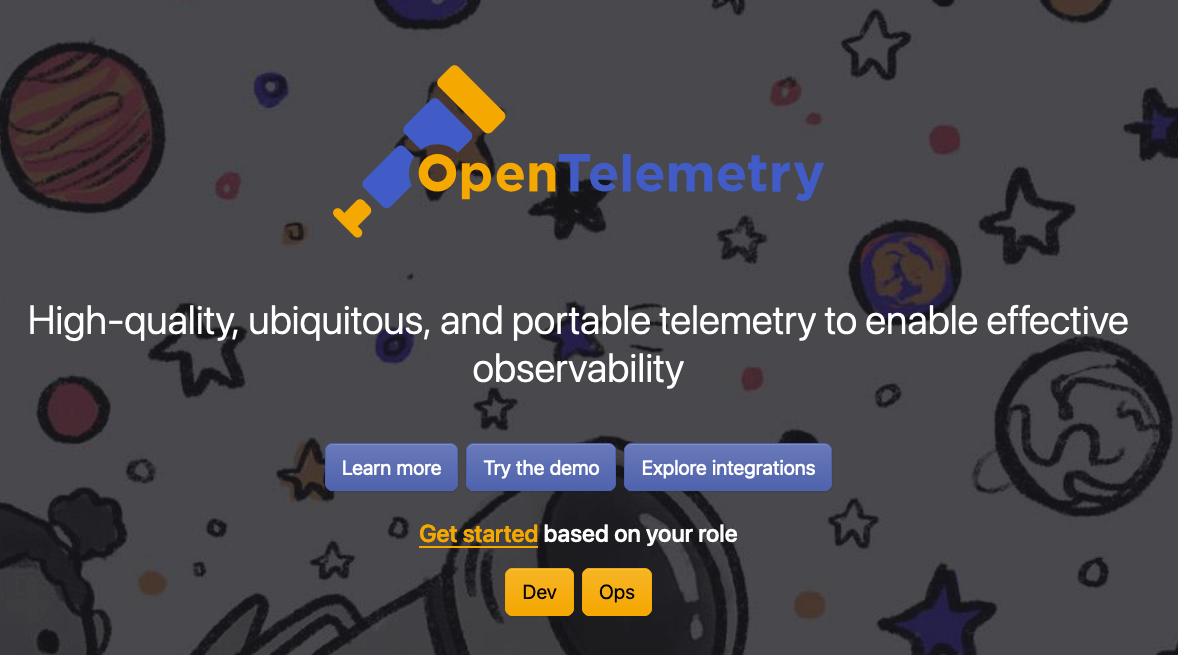
\includegraphics[width=0.7\linewidth]{Images/opentelemetry}
			\label{fig:opentelemetry}
		\end{figure}
	\end{frame}
	
	\begin{frame}
		\begin{figure}
			\centering
			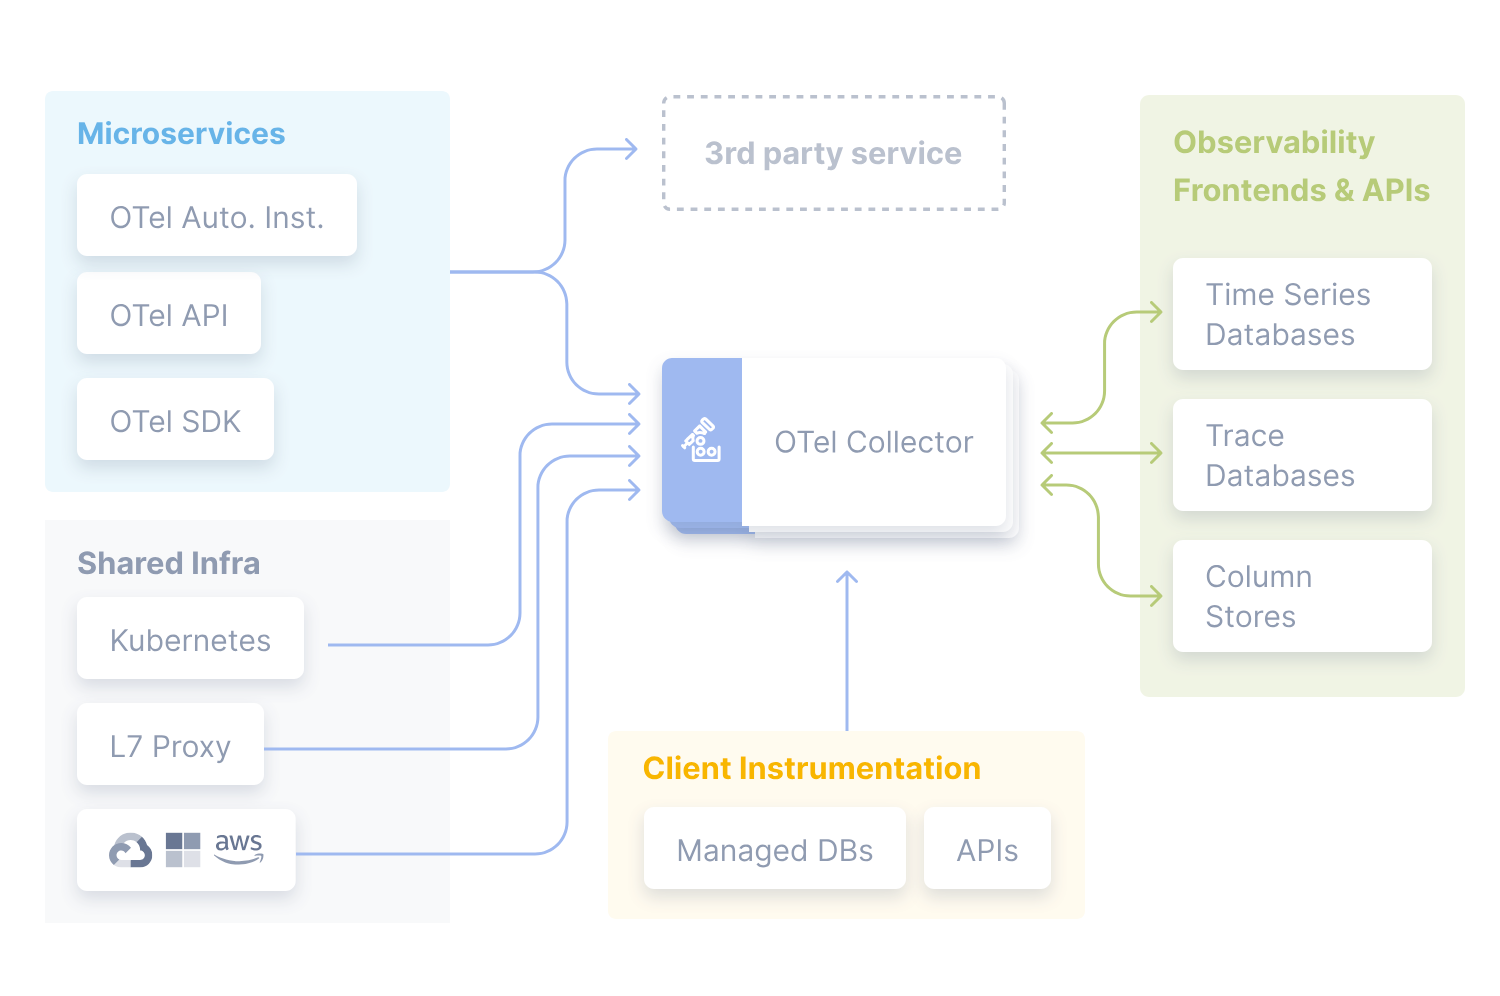
\includegraphics[width=0.8\linewidth]{Images/otelcollector}
			\label{fig:otelcollector}
		\end{figure}
	\end{frame}
	
	\begin{frame}
		\begin{figure}
			\centering
			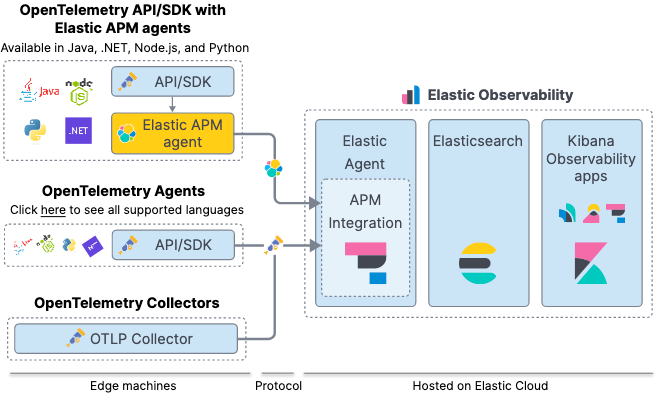
\includegraphics[width=0.8\linewidth]{Images/elasticotel}
			\label{fig:elasticotel}
		\end{figure}
	\end{frame}
	
	\begin{frame}
		\begin{figure}
			\centering
			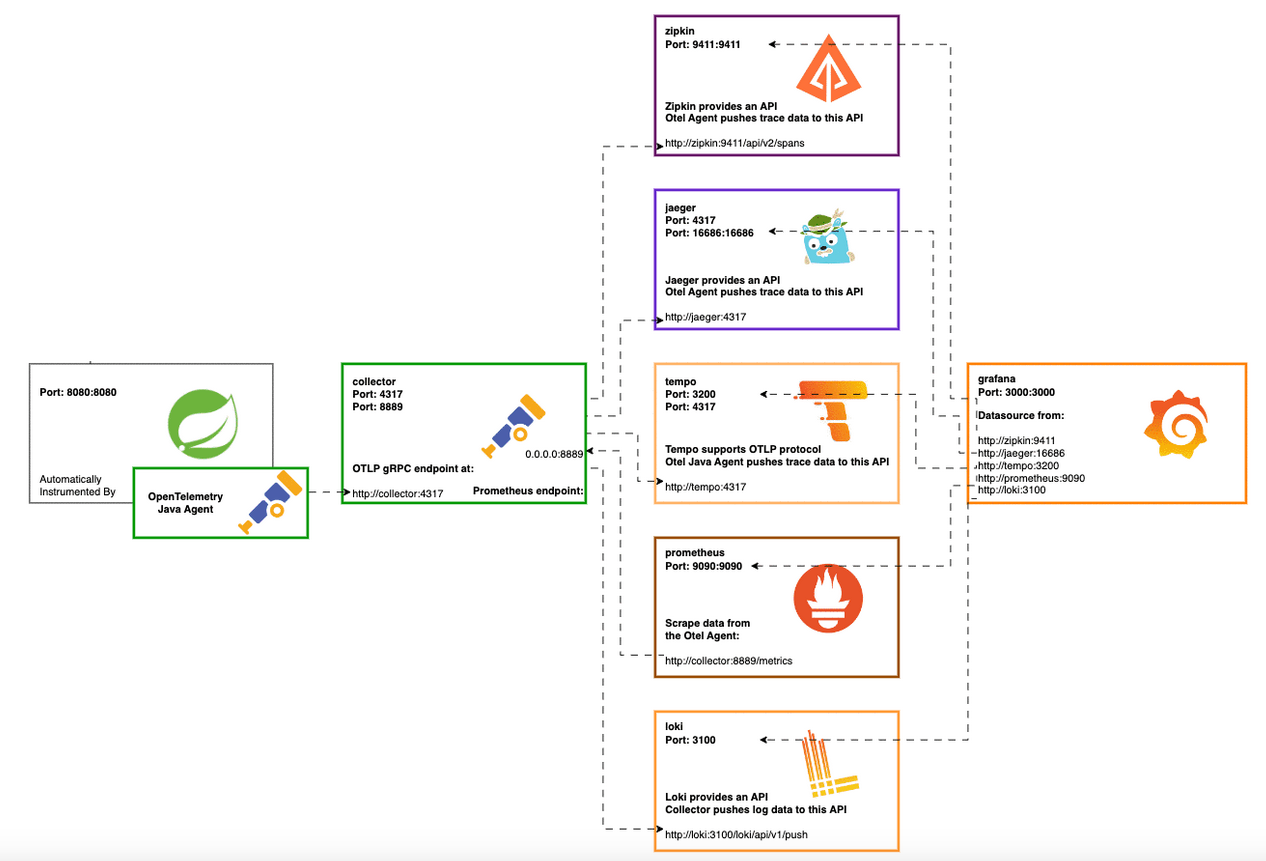
\includegraphics[width=0.8\linewidth]{Images/springboot}
			\label{fig:springboot}
		\end{figure}
	\end{frame}
	
	{
		\usebackgroundtemplate{
\includegraphics[width=\paperwidth]{Images/separador}}
		\setbeamercolor{normal text}{fg=white}
		\setbeamercolor{frametitle}{fg=red}
		\usebeamercolor[fg]{normal text}
		\section{Ejemplo}
	}
	
	\begin{frame}
		\begin{figure}
			\centering
			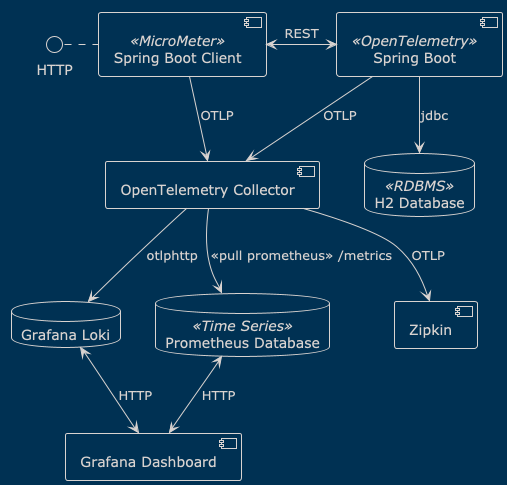
\includegraphics[width=0.5\linewidth]{Images/otel}
			\label{fig:otel}
		\end{figure}
	\end{frame}
	\begin{frame}{Víctor Orozco}
		\begin{columns}[T] % contents are top vertically aligned
			
			\begin{column}[T]{4cm} % alternative top-align that's better for graphics
				\begin{figure}
					\centering
					
\includegraphics[width=0.8\linewidth]{Images/logos}
				\end{figure}
			\end{column}
			\begin{column}[T]{6cm} % each column can also be its own environment
				\begin{itemize}
					\item vorozco@nabenik.com
					\item \href{https://twitter.com/tuxtor}{@tuxtor}
					\item \href{https://vorozco.com}{https://vorozco.com}
					\item \href{https://tuxtor.shekalug.org}{https://tuxtor.shekalug.org}
				\end{itemize}
				\begin{center}
					
\includegraphics[width=0.1\linewidth]{Images/cclogo}
					\\
					This work is licensed under Creative Commons Attribution-NonCommercial-ShareAlike 3.0 Guatemala (CC BY-NC-SA 3.0 GT).
				\end{center}
			\end{column}
		\end{columns}
	\end{frame}
	
	
\end{document}
